\documentclass[11pt]{book}

\usepackage{epsfig}
\usepackage{html}
\usepackage{hypre}
\usepackage{makeidx}
\usepackage{graphicx}

%=============================================================================
% Preamble:
%=============================================================================

% set margins
\setlength{\oddsidemargin}{0in}
\setlength{\evensidemargin}{0in}
\setlength{\textwidth}{6.5in}
\setlength{\topmargin}{0in}
\setlength{\textheight}{8.0in}

% define various commands and macros

% define the version number
% NOTE: this is automatically generated from another file in hypre
\def\HYPREVersion{2.4.0b}
\def\HYPREVersionDate{2008/08/08}


% write out the index entries in the `.idx' file
\makeindex

%=============================================================================
% Body:
%=============================================================================

\begin{document}

%=============== Title Page

\begin{TitlePage}

\Title{\hypre{} User's Manual: Draft}
\SubTitle{Software Revision: \HYPREVersion}
\SubTitle{Date: \HYPREVersionDate}
\vfill
\begin{center}
\InsertGraphics{hypre_wiw}{width=.7\textwidth}
\end{center}
\vfill
\Author{%
Center for Applied Scientific Computing\\
Lawrence Livermore National Laboratory
}

\end{TitlePage}

%=============== Copyright Page

\begin{CopyrightPage}
\noindent
Copyright (c) 2006   The Regents of the University of California.
Produced at the Lawrence Livermore National Laboratory.
Written by the HYPRE team, (hypre-users@llnl.gov), UCRL-CODE-222953.
All rights reserved.

\vspace{1em}\noindent
This notice is required to be provided under our contract with the U.S. 
Department of Energy (DOE). This work was produced at the University of 
California, Lawrence Livermore National Laboratory under Contract No. W7405-ENG-48 with the DOE.
 
\vspace{1em}\noindent
Neither the United States Government nor the University of California nor any 
of their employees, makes any warranty, express or implied, or assumes any 
liability or responsibility for the accuracy, completeness, or usefulness of any 
information, apparatus, product, or process disclosed, or represents that its use 
would not infringe privately-owned rights. 

\vspace{1em}\noindent
Also, reference herein to any specific commercial products, process, or 
services by trade name, trademark, manufacturer or otherwise does not 
necessarily constitute or imply its endorsement, recommendation, or favoring by 
the United States Government or the University of California. The views and 
opinions of authors expressed herein do not necessarily state or reflect those of 
the United States Government or the University of California, and shall not be 
used for advertising or product endorsement purposes. 

\vspace{1em}\noindent
This file is part of HYPRE (see http://www.llnl.gov/CASC/hypre/).
Please see the COPYRIGHT\_and\_LICENSE file for the copyright notice, 
disclaimer and the GNU Lesser General Public License.

\vspace{1em}\noindent
This program is free software; you can redistribute it and/or modify it
under the terms of the GNU General Public License (as published by the Free
Software Foundation) version 2.1 dated February 1999.
  
\vspace{1em}\noindent
This program is distributed in the hope that it will be useful, but WITHOUT
ANY WARRANTY; without even the IMPLIED WARRANTY OF MERCHANTABILITY or
FITNESS FOR A PARTICULAR PURPOSE.  See the terms and conditions of the
GNU General Public License for more details.

\vspace{1em}\noindent
You should have received a copy of the GNU Lesser General Public License
along with this program; if not, write to the Free Software Foundation,
Inc., 59 Temple Place, Suite 330, Boston, MA 02111-1307 USA


\vspace{1em}\noindent
UCRL-MA-137155 DR
\end{CopyrightPage}

%=============== Table of Contents

\pagenumbering{roman}
\tableofcontents
\cleardoublepage
\pagenumbering{arabic}

%=============== Include Chapters


%==========================================================================

\chapter{Introduction}
\label{Introduction}

\hypre{} is a software library for solving large, sparse linear
systems of equations on massively parallel computers.  The library was
created with the primary goal of providing users with advanced
parallel preconditioners.  Issues of robustness, ease of use,
flexibility, and interoperability also play an important role.

%==========================================================================

\section{Features}
\label{Features}

\begin{itemize}

\item
{\bf Scalable preconditioners provide efficient solution on today's
and tomorrow's systems:} \hypre{} contains several families of
preconditioner algorithms focused on the scalable solution of very
large sparse linear systems. \hypre{} includes ``grey-box'' algorithms
that use more than just the matrix to solve certain classes of
problems more efficiently than general-purpose libraries. This
includes algorithms such as structured multigrid and element-based
algebraic multigrid.

\item
{\bf Suite of common iterative methods provides options for a spectrum
of problems:} \hypre{} provides several of the most commonly used
Krylov-based iterative methods to be used in conjunction with its
scalable preconditioners. This includes methods for nonsymmetric
systems such as GMRES and methods for symmetric matrices such as
Conjugate Gradient.

\item
{\bf Intuitive grid-centric interfaces obviate need for complicated
data structures and provide access to advanced solvers:} \hypre{} has
made a major step forward in usability from earlier generations of
sparse linear solver libraries in that users do not have to learn
complicated sparse matrix data structures.  Instead, \hypre{} does the
work of building these data structures for the user through a variety
of interfaces, each appropriate to different classes of users.  These
include stencil-based structured/semi-structured interfaces most
appropriate for finite-difference applications; a finite-element based
unstructured interface; and a linear-algebra based interface.  Each
interface provides access to several solvers without the need to write
new interface code.

\item
{\bf User options accommodate beginners through experts:} \hypre{}
allows a spectrum of expertise to be applied by users. The beginning
user can get up and running with a minimal amount of effort. More
expert users can take further control of the solution process through
various parameters.

\item
{\bf Configuration options to suit your computing system:} \hypre{}
utilizes the GNU Autoconf package to allow simple and flexible
installation on a wide variety of computing systems.  Users can tailor
the installation to match their computing system. Options include
debug and optimized modes, the ability to change required libraries
such as MPI and BLAS, a sequential mode, and modes enabling threads
for certain solvers.  On most systems, however, \hypre{} can be built
by simply typing \kbd{configure} followed by \kbd{make}.

\item
{\bf Interfaces in multiple languages provide greater flexibility for
applications:} \hypre{} contains interfaces for both Fortran and C
users.

\end{itemize}

%==========================================================================

\section{Assumptions and Limitations}

\begin{itemize}

\item
{\bf \hypre{} is designed for large, sparse, linear systems on
parallel computers.}  Small linear systems, systems that are solvable
on a sequential computer, and dense systems are all better addressed
by other libraries that are designed specifically for them.

\item
{\bf To run in parallel, \hypre{} requires an installation of MPI.}

\item
{\bf Configuration of \hypre{} with threads requires an implementation
of OpenMP.}  Currently, only a subset of \hypre{} is threaded.

\end{itemize}


%==========================================================================
\chapter{Conceptual Interfaces for Inputting Problem Data}
\label{Conceptual Interfaces}

\section{What do we mean by ``conceptual interfaces?''}

\section{Which conceptual interface should I use?}


%==========================================================================
\chapter{Structured Grid Interface}
\label{Structured Grid Interface}

In order to get access to the most efficient and scalable solvers for
scalar structured-grid applications, users should use the
\code{Struct} interface described in this chapter.  This interface
will also provide access (this is not yet supported) to solvers in
\hypre{} that were designed for unstructured-grid applications and
sparse linear systems in general.  These additional solvers are
usually provided via the unstructured-grid interface (\code{FEI}) or
the linear-algebraic interface (\code{IJ}) described in Chapters
\ref{chapter-FEI} and \ref{IJ}.

Figure \ref{fig-fv-grid} gives an example of the type of grid
currently supported by the \code{Struct} interface.  The interface
uses a finite-difference or finite-volume style, and currently
supports only scalar PDEs (i.e., one unknown per gridpoint).
\begin{figure}
\centering
\includegraphics[width=4in]{fv_grid.eps}
\caption{%
An example 2D structured grid, distributed accross two processors.}
\label{fig-fv-grid}
\end{figure}

There are four basic steps involved in setting up the linear system
to be solved:
\begin{enumerate}
\item set up the grid,
\item set up the stencil,
\item set up the matrix,
\item set up the right-hand-side vector.
\end{enumerate}
To describe each of these steps in more detail, consider solving the
2D Laplacian problem
\begin{equation}\label{eqn-laplacian}
\left \{
\begin{array}{ll}
\nabla^2 u = f , & \mbox{in the domain}, \\
u = 0,           & \mbox{on the boundary}.
\end{array}
\right .
\end{equation}
Assume (\ref{eqn-laplacian}) is discretized using standard 5-pt
finite-volumes on the uniform grid pictured in \ref{fig-fv-grid}, and
assume that the problem data is distributed across two processes as
depicted.

%==========================================================================

\section{Setting Up the Grid}
\label{Setting Up the Grid}

The grid is described via a global {\em index space}, i.e., via
integer tuples (triples in 3D).  The integers may have any value,
negative or positive.  The global indexes allow \hypre{} to discern
how data is related spatially, and how it is distributed across the
parallel machine.  Each process describes that portion of the grid
that it ``owns'', one {\em box} at a time.  For example, in the
figure, the global grid can be described in terms of three boxes, two
owned by process 0, and one owned by process 1.  A box is described in
terms of a lower and upper index.

On process 0, the following code will set up the grid shown in the
figure (the code for process 1 is similar).
\begin{display}
\begin{verbatim}

HYPRE_StructGrid  grid;
int               ilower[2][2] = {{-3, 1}, {0, 1}};
int               iupper[2][2] = {{-1, 2}, {2, 4}};

HYPRE_StructGridCreate(MPI_COMM_WORLD, 2, &grid);

HYPRE_StructGridSetExtents(grid, ilower[0], iupper[0]);
HYPRE_StructGridSetExtents(grid, ilower[1], iupper[1]);

HYPRE_StructGridAssemble(grid);

\end{verbatim}
\end{display}
The \code{HYPRE_StructGridCreate()} routine creates an empty 2D grid
object that lives on the \code{MPI_COMM_WORLD} communicator.  The
\code{HYPRE_StructGridSetExtents()} routine adds a new box to the grid.
The \code{HYPRE_StructGridAssemble()} routine is a collective call
(i.e., must be called on all processes), and finalizes the grid
assembly, making the grid ``ready to use''.

%==========================================================================

\section{Setting Up the Stencil}
\label{Setting Up the Stencil}

The geometry of the discretization stencil is described by an array of
integer tuples in 2D (triples in 3D), each representing a relative
offset (in index space) from some gridpoint on the grid.  For example,
the geometry of the 5-pt stencil for the example problem being
considered can be represented in the following way:
\begin{equation}\label{eqn-stencil-description}
\left [
\begin{array}{ccc}
        & ( 0, 1) &         \\
(-1, 0) & ( 0, 0) & ( 1, 0) \\
        & ( 0,-1) &        
\end{array}
\right ]
\equiv
\left [
\begin{array}{ccc}
    & S_4 &     \\
S_1 & S_0 & S_2 \\
    & S_3 &    
\end{array}
\right ] .
\end{equation}
In (\ref{eqn-stencil-description}), the $(0,0)$ entry represents the
``center'' coefficient, and is the 0th entry in the array ($S_0$).
The $(0,-1)$ entry represents the ``south'' coefficient, and is the
3rd entry in the array ($S_3$).  And so on.

On process 0 or 1, the following code will set up the stencil in
(\ref{eqn-stencil-description}).  The stencil must be the same on all
processes.
\begin{display}
\begin{verbatim}

HYPRE_StructStencil  stencil;
int                  offsets[5][2] = {{0,0}, {-1,0}, {1,0}, {0,-1}, {0,1}};
int                  s;

HYPRE_StructStencilCreate(2, 5, &stencil);

for (s = 0; s < 5; s++)
{
   HYPRE_StructStencilSetElement(stencil, s, offsets[s]);
}

\end{verbatim}
\end{display}
The \code{HYPRE_StructStencilCreate()} routine creates an empty 2D,
5-pt stencil object.  The \code{HYPRE_StructStencilSetElement()}
routine defines the geometry of the stencil and assigns the array
numbers for each of the stencil entries.  None of the calls are
collective calls.

%==========================================================================

\section{Setting Up the Matrix}
\label{Setting Up the Matrix}

The matrix is set up in terms of the grid and stencil objects
described in Sections
\ref{Setting Up the Grid} and \ref{Setting Up the Stencil}.
The coefficients associated with each stencil entry will typically
vary from gridpoint to gridpoint, but in the example problem being
considered, they are as follows over the entire grid (except at
boundaries; see below):
\begin{equation}\label{eqn-stencil-laplacian}
\left [
\begin{array}{ccc}
    & -1 &    \\
 -1 &  4 & -1 \\
    & -1 &    
\end{array}
\right ] .
\end{equation}

On process 0, the following code will set up matrix values associated
with the center ($S_0$) and south ($S_3$) stencil entries in
(\ref{eqn-stencil-description}) / (\ref{eqn-stencil-laplacian})
(boundaries are ignored here temporarily).
\begin{display}
\begin{verbatim}

HYPRE_StructMatrix  A;
double              values[36];
int                 stencil_indices[2] = {0,3};
int                 i;

HYPRE_StructMatrixCreate(MPI_COMM_WORLD, grid, stencil, &A);
HYPRE_StructMatrixInitialize(A);

for (i = 0; i < 36; i += 2)
{
   values[i]   =  4.0;
   values[i+1] = -1.0;
}

HYPRE_StructMatrixSetBoxValues(A, ilower[0], iupper[0], 2,
                               stencil_indices, values);
HYPRE_StructMatrixSetBoxValues(A, ilower[1], iupper[1], 2,
                               stencil_indices, values);

/* set boundary conditions */
...

HYPRE_StructMatrixAssemble(A);

\end{verbatim}
\end{display}
The \code{HYPRE_StructMatrixCreate()} routine creates an empty matrix
object.  The \code{HYPRE_StructMatrixInitialize()} routine indicates
that the matrix coefficients (or values) are ready to be set.  This
routine may or may not involve the allocation of memory for the
coefficient data, depending on the implementation.  The optional
\code{Set} routines mentioned later in this chapter and in the
Reference Manual, should be called before this step.  The
\code{HYPRE_StructMatrixSetBoxValues()} routine sets the matrix
coefficients for some set of stencil entries over the gridpoints in
some box.  Note that the box need not correspond to any of the boxes
used to create the grid, but values should be set for all gridpoints
that this process ``owns''.  The \code{HYPRE_StructMatrixAssemble()}
routine is a collective call (i.e., must be called on all processes),
and finalizes the matrix assembly, making the matrix ``ready to use''.

Matrix coefficients that reach outside of the boundary should be set
to zero.  For efficiency reasons, \hypre{} does not do this
automatically.  The most natural time to insure this is when the
boundary conditions are being set, and this is most naturally done
after the coefficients on the grid's interior have been set.  For
example, during the implementation of the Dirichlet boundary condition
on the lower boundary of the grid in Figure \ref{fig-fv-grid}, the
``south'' coefficient must be set to zero.  To do this on process 0,
the following code could be used:
\begin{display}
\begin{verbatim}

int  ilower[2] = {-3, 1};
int  iupper[2] = { 2, 1};

/* create matrix and set interior coefficients */
...

/* implement boundary conditions */
...

for (i = 0; i < 12; i++)
{
   values[i] =  0.0;
}

i = 3;
HYPRE_StructMatrixSetBoxValues(A, ilower, iupper, 1, &i, values);

/* complete implementation of boundary conditions */
...

\end{verbatim}
\end{display}

%==========================================================================

\section{Setting Up the Right-Hand-Side Vector}
\label{Setting Up the Right-Hand-Side Vector}

The right-hand-side vector is set up similarly to the matrix set up
described in Section \ref{Setting Up the Matrix} above.  The main
difference is that there is no stencil (note that a stencil currently
does appear in the interface, but this will eventually be removed).

On process 0, the following code will set up the right-hand-side
vector values.
\begin{display}
\begin{verbatim}

HYPRE_StructVector  b;
double              values[18];
int                 i;

HYPRE_StructVectorCreate(MPI_COMM_WORLD, grid, &b);
HYPRE_StructVectorInitialize(b);

for (i = 0; i < 18; i++)
{
   values[i]   =  0.0;
}

HYPRE_StructVectorSetBoxValues(b, ilower[0], iupper[0], values);
HYPRE_StructVectorSetBoxValues(b, ilower[1], iupper[1], values);

HYPRE_StructVectorAssemble(b);

\end{verbatim}
\end{display}

The \code{HYPRE_StructVectorCreate()} routine creates an empty vector
object.  The \code{HYPRE_StructVectorInitialize()} routine indicates
that the vector coefficients (or values) are ready to be set.  This
routine follows the same rules as its corresponding \code{Matrix}
routine.  The \code{HYPRE_StructVectorSetBoxValues()} routine sets the
vector coefficients over the gridpoints in some box, and again,
follows the same rules as its corresponding \code{Matrix} routine.
The \code{HYPRE_StructVectorAssemble()} routine is a collective call
(i.e., must be called on all processes), and finalizes the vector
assembly, making the vector ``ready to use''.

%==========================================================================

\section{Symmetric Matrices}
\label{Symmetric Matrices}

Some solvers and matrix storage schemes provide capabilities for
significantly reducing memory usage when the coefficient matrix is
symmetric.  In this situation, each off-diagonal coefficient appears
twice in the matrix, but only one copy needs to be stored.  The
\code{Struct} interface provides support for matrix and solver
implementations that use symmetric storage via the
\code{HYPRE_StructMatrixSetSymmetric()} routine.

To describe this in more detail, consider again the 5-pt finite-volume
discretization of (\ref{eqn-laplacian}) on the grid pictured in Figure
\ref{fig-fv-grid}.  Because the discretization is symmetric, only half
of the off-diagonal coefficients need to be stored.  To turn symmetric
storage on, the following line of code needs to be inserted somewhere
between the \code{HYPRE_StructMatrixCreate()} and
\code{HYPRE_StructMatrixInitialize()} calls.
\begin{display}
\begin{verbatim}

HYPRE_StructMatrixSetSymmetric(A, 1);

\end{verbatim}
\end{display}
Note that symmetric storage may or may not actually be used, depending
on the underlying storage scheme.  Currently in \hypre{}, symmetric
storage is always used when indicated.

To most efficiently utilize the \code{Struct} interface for symmetric
matrices, notice that only half of the off-diagonal coefficients need
to be set.  To do this for the example being considered, we simply
need to redefine the 5-pt stencil of Section
\ref{Setting Up the Stencil} to an ``appropriate'' 3-pt stencil, then
set matrix coefficients (as in Section \ref{Setting Up the Matrix})
for these three stencil elements {\em only}.  For example, we could
use the following stencil
\begin{equation}\label{eqn-symmetric-stencil}
\left [
\begin{array}{ccc}
 & ( 0, 1) &         \\
 & ( 0, 0) & ( 1, 0) \\
 &         &        
\end{array}
\right ]
\equiv
\left [
\begin{array}{ccc}
 & S_2 &     \\
 & S_0 & S_1 \\
 &     &    
\end{array}
\right ] .
\end{equation}
This 3-pt stencil provides enough information to recover the full 5-pt
stencil geometry and associated matrix coefficients.

%==========================================================================

%==========================================================================
\chapter{The IJ Linear System Interface}
\label{IJ}

The {\bf IJ linear system (IJ)} interface is the lowest common
denominator
for enumeration of an {\bf unaugmented} linear system of equations
to be solved by {\slshape hypre} and cooperative packages.
No underlying assumptions are made about the sparsity pattern of
a linear system passed through the IJ interface.
Like all Hypre interfaces, it is designed
to insulate the user from underlying implementation details.

Just to define an {\bf augmented} linear system, an example would be
a linear system plus the stiffness matrices from which the matrix
coefficients are assembled in a finite element discretization.
It contains more information than just the linear system
of equations.

One would typically use the IJ interface to enumerate the linear
system originating from an unstructured grid PDE discretization.
However, the interface can be used for discretizations from more
structured grids, with consequent solver inefficiencies from lack
of built-in sparsity assumptions.

IJ Matrix interface calls facilitate creation and destruction of 
interface objects, enumeration of rows and blocks of
linear system coefficients, and determination and querying of
underlying linear system data structure formats.  Hypre supports
multiple underlying data structure formats in order to cooperate
with packages such as PETSc and ISIS, as well as for convenience
to the {\slshape hypre} solver developer.
One format is abbreviated {\bf ParCSR}, meaning {\bf Par}allel
{\bf C}ompressed {\bf S}parse {\bf R}ow.  Another format
is DistributedMatrix.

Currently, {\slshape hypre} solvers which operate directly on linear
systems passing through the IJ interface have either
ParCSR (interface) implementations, or DistributedMatrix
implementations.

\section{IJ Matrix Interface}

\section{IJ Vector Interface}

Fortran implementation (temporarily):

      call HYPRE_IJVectorCreate(rad_comm, hypre_b, global_number_pts,
     &                          ierr)

      call HYPRE_IJVectorSetLocalStorageTy(hypre_b, HYPRE_PARCSR, ierr)

Processors can be informed about distribution of unknowns over processors,

      call HYPRE_IJVectorSetLocalPartition(hypre_b, domain_pt_start,
     &                                     next_domain_pt_start,
     &                                     ierr)

and then all processors must agree upon the distribution, ...

      call HYPRE_IJVectorAssemble(hypre_b, ierr)                     .

Memory space is then allocated for the vector components that must
be handled on the processor, ...

      call HYPRE_IJVectorInitialize(hypre_b, ierr)                   .

      call HYPRE_IJVectorCreate(rad_comm, hypre_x, global_number_pts,
     &                          ierr)

      call HYPRE_IJVectorSetLocalStorageTy(hypre_x, HYPRE_PARCSR,
     &                                     ierr)

      call HYPRE_IJVectorSetLocalPartition(hypre_x, domain_pt_start,
     &                                     next_domain_pt_start,
     &                                     ierr)

      call HYPRE_IJVectorAssemble(hypre_x, ierr)

      call HYPRE_IJVectorInitialize(hypre_x, ierr)


Vector components can be placed into underlying Hypre formats either
in contiguous subsets, ...

      call HYPRE_IJVectorSetLocalCompsInBl(hypre_b,
     &                                     domain_pt_start,
     &                                     next_domain_pt_start-1,
     &                                     ii,y,ierr)

      call HYPRE_IJVectorSetLocalCompsInBl(hypre_x,
     &                                     domain_pt_start,
     &                                     next_domain_pt_start-1,
     &                                     ii,x,ierr)

or in indexed subsets

      call HYPRE_IJVectorSetLocalComps(hypre_b,
     &                                 domain_pt_start,
     &                                 next_domain_pt_start-1,
     &                                 ii,y,ierr)

      call HYPRE_IJVectorSetLocalComps(hypre_x,
     &                                 domain_pt_start,
     &                                 next_domain_pt_start-1,
     &                                 ii,x,ierr)                   .

After the solver is finished, vector components can be extracted from
a contiguous subset of components, ...

      call HYPRE_IJVectorGetLocalCompsInBl(hypre_x,
     &                                     domain_pt_start,
     &                                     next_domain_pt_start-1,
     &                                     ii, x, ierr)

or from an indexed subset of components, ...

      call HYPRE_IJVectorGetLocalCompsInBl(hypre_x,
     &                                     num_values,
     &                                     ii, x_indices, x, ierr)  .

One can also add to vector components that are already set.


\chapter{Finite Element Interface}
\label{ch-FEI}

\section{Introduction}

User applications access the \hypre{} linear solvers via a pipeline of
two interfaces - user to finite element interface (called {\sf FEI}),
and the finite element to linear solver interface (called 
{\sf LinearSystemCore}). The purpose of {\sf FEI} is to allow users 
to submit the global matrices in the form of element connectivities, 
element stiffness matrices, element loads, and boundary conditions. 
These element information are processed by an implementation of the 
{\sf FEI} (see \cite{FEI-ref}) which loads the global matrix and right
hand side vectors to the linear solver libraries via the 
{\sf LinearSystemCore} interface.
The {\sf LinearSystemCore} interface also facilitates interfacing 
multiple linear system solver packages (such as PetSC or Aztec)
with little change in the user code.

The specification of the {\sf FEI} and its implementation was first
developed at Sandia. A simplified implementation has been implemented
at LLNL in \hypre{}'s finite element module. In the next section, we 
describe the basic {\sf FEI} functions and a sample program to 
demonstrate how to use them. 
%A brief description of \hypre{}'s 
%internal data structure and solver capabilities is presented in 
%Section 5.3.  Associated with \hypre{}'s finite element interface is 
%an FE-based gray-box multilevel preconditioning module called 
%{\sf MLI} which provides fast multilevel preconditioners.
%A description of the {\sf MLI} is given in Section 5.4.
%In Section 5.5, we describe the available options for using \hypre{}'s
%rich solver capabilities. 
Users who prefer to create their own finite
element packages but would like to use the \hypre{} solvers can link their
packages to \hypre{} via the {\sf LinearSystemCore}. A description
of this interface is given in Section 4.3.  Finally, some installation 
and usage issues are discussed in Section 4.4.

\section{A Brief Description of The Finite Element Interface}

Embedded in application finite element codes are data structures
storing element connectivities, element stiffness matrices, element
loads, boundary conditions, nodal coordinates, etc. An implicit finite
element problem can be solved by assembling the global stiffness matrix
and the corresponding right hand side vector, and then calling linear
solver to calculate the solution. The first step in this process is 
thus to instantiate an {\sf FEI} object by
\begin{tabbing}
\hspace{0.5in} \= {\sf feiPtr = new FEI\_Implementation(mpiComm);}
\end{tabbing}
where {\sf mpiComm} is an MPI communicator (e.g. {\sf MPI\_COMM\_WORLD}).
Next, various finite element information need to be sent into the {\sf FEI}
object.

The first entity to be submitted to the {\sf FEI} is {\it field} information. 
A {\it field} has an identifier called {\it fieldID} and a rank or
{\it fieldSize} (number of degree of freedom). For example, for a simple
3D incompressible Navier Stokes equation, the nodal variable is the velocity
vector which has $3$ degrees of freedom; and the element variable (constant
over the element) is the pressure (scalar). If these are the only variables,
and if we assign {\it fieldID} $7$ and $8$ to them, respectively, then the
finite element field information can be set up by
\begin{tabbing}
\hspace{0.5in} \= {\sf nFields = 2;} \\
               \> {\sf fieldID = new int[nFields];} \\
               \> {\sf fieldID[0] = $7$; /* velocity vector */} \\
               \> {\sf fieldID[1] = $8$; /* pressure */} \\
               \> {\sf fieldSize = new int[nFields];} \\
               \> {\sf fieldSize[0] = $3$; /* velocity vector */} \\
               \> {\sf fieldSize[1] = $1$; /* pressure */ } \\
               \> {\sf feiPtr$->$initFields(nFields, fieldSize, fieldID);}
\end{tabbing}

Once the field information has been established, we are ready to initialize
an element block. An element block is characterized by the block identifier,
the number of elements, the number of nodes per element, the nodal fields 
and the element fields (fields that have been defined previously). Suppose 
we use $1000$ hexahedral elements in the element block $0$, the setup 
consists of
\begin{tabbing}
\hspace{0.5in} \= {\sf elemBlkID = 0;} \\
               \> {\sf nElems = 1000;} \\
               \> {\sf elemNNodes = 8; /* number of nodes per element */} \\
               \> {\sf nodeNFields = 1; /* nodal field - velocity */} \\
               \> {\sf nodeFieldIDs = new[nodeNFields];} \\
               \> {\sf nodeFieldIDs[0] = fieldID[0]; /* velocity */ } \\
               \> {\sf elemNFields = 1; /* element field - pressure */} \\
               \> {\sf elemFieldIDs = new[elemNFields];} \\
               \> {\sf elemFieldIDs[0] = fieldID[1]; /* pressure */ } \\
 \> {\sf feiPtr$->$initElemBlock(elemBlkID, nElems, elemNNodes, nodeNFields, nodeFieldIDs,}\\
 \> \hspace{1.0in} {\sf elemNFields, elemFieldIDs, 0);} 
\end{tabbing}
The last argument is to specify how the dependent variables are arranged in
the element matrices. A value of $0$ indicates that each variable is to be
arranged in a separate block (as opposed to interleaving).

In a parallel environment, each processor has one or more element blocks.
Unless the element blocks are all disjoint, some of the element blocks
share a common set of nodes on the subdomain boundaries. To facilitate
setting up interprocessor communications, shared nodes between subdomains
on different processors are to be identified and sent to the {\sf FEI}.
Hence, each node in the whole domain is assigned a unique global
identifier. The shared node list on each processor contains a subset
of the global node list
corresponding to the local nodes that are shared with the other processors.
The syntax for setting up the shared nodes is
\begin{tabbing}
\hspace{0.5in} \= {\sf feiPtr$->$initSharedNodes(nShared, sharedIDs, sharedLengs, sharedProcs);}
\end{tabbing}
This completes the initialization phase, and a completion signal is sent to
the {\sf FEI} via
\begin{tabbing}
\hspace{0.5in} \= {\sf feiPtr$->$initComplete();}
\end{tabbing}

Next we begin the {\it load} phase. The first entity for loading is the
nodal boundary conditions. Here we need to specify the number of boundary
equations and the boundary values given by {\sf alpha, beta}, and {\sf gamma}.  Depending whether the boundary conditions are Dirichlet, Neumann, or mixed,
the three values should be passed into the {\sf FEI} accordingly. 

The element stiffness matrices are to be loaded in the next step. We need
to specify the element number $i$, the element block to which element $i$
belongs, the element connectivity information, the element load, and the
element matrix format. The element connectivity specifies a set of $8$ node
global IDs (for hexahedral elements), and the element load is the load or
force for each degree of freedom.  The element format specifies how the
equations are arranged (similar to the interleaving scheme mentioned above).
The calling sequence for loading element stiffness matrices is
\begin{tabbing}
\hspace{0.5in} \= {\sf for (iE = 0; iE < nElems; iE++)} \\
 \> \hspace{0.5in} {\sf feiPtr$->$sumInElem(elemBlkID, elemID, elemConn[iE], elemStiff[iE],} \\
 \> \hspace{1.5in} {\sf elemLoads[iE], elemFormat);}
\end{tabbing}
Again, to complete the loading phase, a completion signal is sent to 
the {\sf FEI} via
\begin{tabbing}
\hspace{0.5in} \= {\sf feiPtr$->$loadComplete();}
\end{tabbing}
 
Now the global stiffness matrix and the corresponding right hand side
have been assembled. Before the linear system is solved, a number of 
solver parameters have to be passed into the {\sf FEI}. A detailed description
of the solver parameters is given in Section 3. An example is given below
\begin{tabbing}
\hspace{0.5in} \= {\sf nParams = 5;} \\
               \> {\sf paramStrings = new char*[nParams];} \\
               \> {\sf for (i = 0; i < nParams; i++) }\\
               \> \hspace{0.5in} {\sf paramStrings[i] = new char[100];} \\
               \> {\sf strcpy(paramStrings[0], "solver cg");} \\
               \> {\sf strcpy(paramStrings[1], "preconditioner diag");} \\
               \> {\sf strcpy(paramStrings[2], "maxiterations 100");} \\
               \> {\sf strcpy(paramStrings[3], "tolerance 1.0e-6");} \\
               \> {\sf strcpy(paramStrings[4], "outputLevel 1");} \\
               \> {\sf feiPtr$->$parameters(nParams, paramStrings);} 
\end{tabbing}

To solve the linear system of equations, we call
\begin{tabbing}
\hspace{0.5in} \= {\sf feiPtr$->$solve(\&status);}
\end{tabbing}
where {\sf status} is returned from the {\sf FEI} indicating whether
the solve is successful. Finally, the solution can be retrieved by
\begin{tabbing}
\hspace{0.5in} \= {\sf feiPtr$->$getBlockNodeSolution(elemBlkID, nNodes, nodeIDList, solnOffsets, solnValues);}
\end{tabbing}
where {\sf solnOffsets[i]} is the index pointing to the first location 
where the variables at node $i$ is returned in {\sf solnValues}.

\section{The LinearSystemCore Interface}

As described before, users who prefer to create their own finite element
interface package can also take advantage of the rich solver capabilities
in \hypre{}. In this section we show how to access {\sf HYPRE\_LinSysCore}'s
internal solver directly.  Users who choose this path need first to 
construct an array (say, {\sf eqnOffsets} describing the matrix row
partitioning across all processors (so {\sf eqnOffsets[p]} and
{\sf eqnOffset[p+1]} have the starting and ending row indices for processor
p). Furthermore, suppose the local submatrix has been constructed as a
compressed sparse row (CSR) matrix in the {\sf ia, ja, val} arrays. 
The following program segment describes the function calls to set up
the internal matrix and solve the linear system.

\begin{tabbing}
\hspace{0.5in} \= {\sf Program Segment} \\[1mm]
\> {\sf startRow = eqnOffsets[mypid];} \\
\> {\sf endRow = eqnOffsets[mypid+1] - 1;} \\
\> {\sf nrows = endRow - startRow + 1} \\
\> {\sf for ( i = startRow; i $<=$ endRow; i++ ) $\{$ } \\
\> \hspace{0.3in} \= {\sf ncnt = ia[i+1] - ia[i];} \\
\> \> {\sf rowLengths[i-startRow] = ncnt;} \\
\> \> {\sf colIndices[i-startRow] = new int[ncnt];} \\
\> \> {\sf k = 0;} \\
\> \> {\sf for (j = ia[i]; j < ia[i+1]; j++) colIndices[i-startRow][k++] = ja[j];}\\
\> \} \\
\> {\sf HYPRE\_LinSysCore\_create(\&lsc, MPI\_COMM\_WORLD);} \\
\> {\sf HYPRE\_setGlobalOffsets(lsc, nrows, NULL, eqnOffsets, NULL);} \\
\> {\sf HYPRE\_setMatrixStructure(lsc, colIndices, rowLengths, NULL, NULL, NULL);} \\
\> {\sf for ( i = startRow; i <= endRow; i++ ) $\{$ } \\
\> \> {\sf ncnt = ia[i+1] - ia[i];} \\
\> \> {\sf HYPRE\_sumIntoSystemMatrix(lsc, i, ncnt, \&val[ia[i]], \&ja[ia[i]]);}\\
\> \> {\sf HYPRE\_sumIntoRHSVector(1, \&rhs[i], \&i);} \\
\> \} \\
\> {\sf HYPRE\_matrixLoadComplete();}\\
\> {\sf strcpy(paramString, "solver gmres");} \\
\> {\sf HYPRE\_parameters(1, \&paramString);} \\
\> {\sf strcpy(paramString, "preconditioner boomeramg");} \\
\> {\sf HYPRE\_parameters(1, \&paramString);} \\
\> {\sf HYPRE\_launchSolver(\&status, \&iterations);}
\end{tabbing}

A list of available functions is given in the following.

\begin{tabbing}
{\sf HYPRE\_LinSysCore\_create(LinSysCore **lsc, MPI\_Comm comm)} \\[1mm]
{\sf HYPRE\_LinSysCore\_destroy(LinSysCore **lsc)} \\[1mm]
{\sf HYPRE\_parameters(LinSysCore *lsc, int nParams, char **params)} \\[1mm]
{\sf HYPRE\_setGlobalOffsets(LinSysCore* lsc, int leng, int* nodeOffsets,} \\
\hspace{1.0in} {\sf int* eqnOffsets, int* blkEqnOffsets)} \\[1mm]
{\sf HYPRE\_setMatrixStructure(LinSysCore *lsc, int** ptColIndices,} \\
\hspace{1.0in} {\sf int* ptRowLengths, int** blkColIndices, int* blkRowLengths, int* ptRowsPerBlkRow)} \\[1mm]
{\sf HYPRE\_resetMatrixAndVector(LinSysCore *lsc, double val)} \\[1mm]
{\sf HYPRE\_resetMatrix(LinSysCore *lsc, double val)} \\[1mm]
{\sf HYPRE\_resetRHSVector(LinSysCore *lsc, double val)} \\[1mm]
{\sf HYPRE\_sumIntoSystemMatrix(LinSysCore *lsc, int numPtRows, const int* ptRows,}\\
\hspace{1.0in} {\sf int numPtCols, const int* ptCols, int numBlkRows, const int* blkRows,} \\
\hspace{1.0in} {\sf int numBlkCols, const int* blkCols, const double* const* values)} \\[1mm]
{\sf HYPRE\_sumIntoRHSVector(LinSysCore *lsc, int num, const double* values, const int* indices)} \\[1mm]
{\sf HYPRE\_matrixLoadComplete(LinSysCore *lsc)} \\[1mm]
{\sf HYPRE\_enforceEssentialBC(LinSysCore *lsc, int* globalEqn, double* alpha,
                             double* gamma, int leng)} \\[1mm]

{\sf HYPRE\_enforceRemoteEssBCs(LinSysCore *lsc,int numEqns,int* globalEqns, int** colIndices,} \\
\hspace{1.0in} {\sf int* colIndLen, double** coefs)} \\[1mm]

{\sf HYPRE\_enforceOtherBC(LinSysCore *lsc, int* globalEqn, double* alpha, double *beta} \\
\hspace{1.0in} {\sf double* gamma, int leng)} \\[1mm]

{\sf HYPRE\_putInitialGuess(LinSysCore *lsc, const int* eqnNumbers,
                          const double* values, int leng)} \\[1mm]
{\sf HYPRE\_getSolution(LinSysCore *lsc, double *answers, int leng)} \\[1mm]

{\sf HYPRE\_getSolnEntry(LinSysCore *lsc, int eqnNumber, double *answer)} \\[1mm]

{\sf HYPRE\_formResidual(LinSysCore *lsc, double *values, int leng)} \\[1mm]

{\sf HYPRE\_launchSolver(LinSysCore *lsc, int *solveStatus, int *iter)} \\[1mm]
\end{tabbing}

\section{HYPRE LinearSystemCore Installation}

The ultimate objective is for application users to have immediate access
to the latest FEI/\hypre{} library files on different computing platforms
via public {\sf lib} directories.  While this feature is forthcoming, careful 
version control is needed for users to keep track of capabilities and bug fixes 
for different installations.  Users who would like to set up the FEI/\hypre{}
on their own should do the following :

\begin{enumerate}

\item obtain the \hypre{} and the Sandia FEI source codes (alternatively, use
      the {\sf FEI} implementation in \hypre{}),
\item compile Sandia's {\sf FEI} (fei-2.5.0) to create the
      {\sf libfei\_base.a} file.
\item compile \hypre{} 
\begin{enumerate}
\item download \hypre{} from the web, ungzip and untar it
\item go into the {\sf linear\_solvers} directory
\item do a 'configure' with the {\sf --with-fei-inc-dir} option set to
      the {\sf FEI} include directory plus other compile options
\item compile with {\sf make install} to create the
      {\sf libHYPRE\_LSI*} file in the {\sf linear\_solvers/hypre/lib}
      directory.
\end{enumerate}
\item call the {\sf FEI} functions in your application code (example given
      previously)
\begin{enumerate}
\item include {\sf cfei\-hypre.h} in your file 
\item include {\sf FEI\_Implementation.h} in your file 
\item make sure your application has an {\sf include} and an {\sf lib} path 
      to the {\sf include} and {\sf lib} directories created above. 
\end{enumerate}

\end{enumerate}

%\subsection{Linking with the library files}

To link the {\sf FEI} and \hypre{} into the executable, the following has to be
attached to the linking command :

\begin{tabbing}
\hspace{0.5in} \= {\sf -L\$$\{$LIBPATHS$\}$ -lfei\_base -lHYPRE\_LSI} 
\end{tabbing}
along with all the other libraries (Note : the order in which the libraries are
listed may be important), where {\sf LIBPATHS} are where 
the \hypre{} and {\sf FEI} libraray files can be found.  

Since some of these library files make calls to LAPACK and BLAS functions, 
the corresponding libraries need to be linked along with (placed after) these 
library files.  
%For example, on the DEC cluster, it suffices to link
%with the {\sf dxml} library, (So {\sf -ldxml} is placed after the above link
%sequence, with {\sf -lm} placed after {\sf -ldxml}.) while the {\it essl}
%library can be used on the blue machine. If {\sf SuperLU} is also needed,
%{\sf -lHYPRE\_superlu} should be placed immediately after {\sf HYPRE\_LSI}.

%\subsection{Some more caveats for application developers}

Building an application executable often requires linking with many different
software packages, and many software packages use some LAPACK and/or BLAS
functions.  In order to alleviate the problem of multiply defined functions
at link time, it is recommended that all software libraries are stripped of
all LAPACK and BLAS function definitions.  These LAPACK and BLAS functions 
should then be resolved at link time by linking with the system LAPACK and
BLAS libraries (e.g. dxml on DEC cluster).  Both \hypre{} and SuperLU were
built with this in mind.  However, some other software library files needed
may have the BLAS functions defined in them.  To avoid the problem of
multiply defined functions, it is recommended that the offending library
files be stripped of the BLAS functions.

%\subsection{Comments about the FEI/\hypre{} Interface and Contacts}

%Comments about \hypre{}'s finite element interface can be directed
%to Charles Tong (925-422-3411, chtong@llnl.gov).


\chapter{Solvers and Preconditioners}
\label{solvers}

The procedure for setup and use of solvers and preconditioners is largely
the same. We will refer to them both as solvers in the sequel except when noted. 
In normal usage, 
the preconditioner is chosen and constructed before the solver,
and then handed to the solver as part of the solver's setup.
In the following, we assume the most common usage pattern in which
a single linear system is set up and then solved with a single righthand
side. We comment later on considerations for other usage patterns.

{\bf Setup:}

\begin{enumerate}

\item
{\bf Pass to the solver the information defining the problem.} In the typical user cycle, the user
has passed this information into a matrix through one of the conceptual interfaces prior to
setting up the solver. In this situation, the problem definition information is then passed to
the solver by passing the constructed matrix into the solver. As described before, the matrix
and solver must be compatible, in that the matrix must provide the services needed by
the solver. Krylov solvers, for example, need only a matrix-vector multiplication. 
Most preconditioners, on the other hand, have additional requirements such as access to the
coefficients of the matrix, e.g. the GetRow function in the \code{HYPRE\_DistributedMatrix} 
class.

\item
{\bf Choose parameters that control construction of the preconditioner/solver.} 
Parameters are chosen through the \code{Set} calls provided by the solver.
As is true throughout \hypre{}, all parameters have reasonable defaults if not chosen.
Note that in \hypre{}, convergence criteria can be chosen after the preconditioner/solver
has been setup.

\item
{\bf Pass the preconditioner to the solver.} For solvers that are not preconditioned, this step
is omitted. The preconditioner is passed through the \code{SetPreconditioner} call. The object passed
in as the preconditioner must be a fully constructed \code{Solver}.

\item
{\bf Set up the solver.} In the procedural C interface for \hypre{}, this is the \code{Setup} call.
In the ESI-compliant interface for \hypre{}, this is the \code{GetConstructedObject} from the
solver builder interface.

\end{enumerate}

At this point, the solver/preconditioner is fully constructed and ready for use. 

{\bf Use:}

\begin{enumerate}

\item
{\bf Set convergence criteria.} Convergence can be controlled by the number of iterations,
as well as various tolerances such as relative residual, preconditioned residual, etc.
Like all parameters, reasonable defaults are used. Generally speaking, Krylov solvers
default to a tolerance-based convergence criteria, while solvers used traditionally as
preconditioners default to convergence based on the number of iterations (usually a single
iteration). Users are free to change these, though care must be taken. Some Krylov solvers,
for example, are not guaranteed to converge unless the preconditioner is a constant operator,
which is only satisfied for iterative methods if a fixed number of iterations
(typically one) is taken.
For these solvers, a preconditioner
with a tolerance-based convergence criteria will not usually work.

\item
{\bf Apply the solver to the right hand side.} For the procedural C interface, this is the 
\code{Solve} function. 
%From the ESI-compliant interface, this is the \code{Apply} function.

\end{enumerate}

%==========================================================================
\chapter{Solvers Available}
\label{Solvers Available}

There are several solvers available in \hypre{}.  Some of them are
listed below.

%==========================================================================
\section{ParaSails}

ParaSails is a parallel implementation of a sparse approximate inverse
preconditioner, using {\em a priori} sparsity patterns and least-squares
(Frobenius norm) minimization.  Symmetric positive definite (SPD) problems
are handled using a factored SPD sparse approximate inverse.  General
(nonsymmetric and/or indefinite) problems are handled with an
unfactored sparse approximate inverse.  It is also possible to
precondition nonsymmetric but definite matrices with a factored, SPD
preconditioner.

ParaSails uses {\em a priori} sparsity patterns that are patterns of powers
of sparsified matrices.  ParaSails also uses a post-filtering technique
to reduce the cost of applying the preconditioner.  
In advanced usage not described here, the pattern of the
preconditioner can also be reused to generate preconditioners for different
matrices in a sequence of linear solves.

For more details about the ParaSails algorithm, see \cite{Chow:1999:APS}.

\subsection{Synopsis}

\begin{display}
\begin{verbatim}
#include "HYPRE_parcsr_ls.h"

int HYPRE_ParaSailsCreate(MPI_Comm comm, HYPRE_Solver *solver, 
  int symmetry);
int HYPRE_ParaSailsSetParams(HYPRE_Solver solver, 
  double thresh, int nlevel, double filter);
int HYPRE_ParaSailsSetup(HYPRE_Solver solver, HYPRE_ParCSRMatrix A,
  HYPRE_ParVector b, HYPRE_ParVector x);
int HYPRE_ParaSailsSolve(HYPRE_Solver solver, HYPRE_ParCSRMatrix A,
  HYPRE_ParVector b, HYPRE_ParVector x);
int HYPRE_ParaSailsStats(HYPRE_Solver solver);
int HYPRE_ParaSailsDestroy(HYPRE_Solver solver);
\end{verbatim}
\end{display}

The accuracy and cost of ParaSails are parameterized by the real {\em thresh}
and integer {\em nlevels} parameters,
$0 \le {\it thresh} \le 1$, $0 \le {\it nlevels}$.
Lower values of {\em thresh}
and higher values of {\em nlevels} lead to more accurate, but more expensive
preconditioners.  More accurate preconditioners are also more expensive
per iteration.  The default values are ${\it thresh} = 0.1$
and ${\it nlevels} = 1$.  The parameters are set using
{\tt HYPRE\_ParaSailsSetParams}.

Mathematically, given a symmetric matrix $A$, the pattern of the
approximate inverse is the pattern of $\tilde{A}^m$ where $\tilde{A}$
is a matrix that has been sparsified from $A$.  The sparsification
is performed by dropping all entries in a symmetrically diagonally scaled $A$
whose values are less than {\em thresh} in magnitude.  The parameter
{\em nlevel} is equivalent to $m+1$.
Filtering is a post-thresholding procedure.
For more details about the algorithm, see \cite{Chow:1999:APS}.

The storage required for the ParaSails preconditioner depends on
the parameters {\em thresh} and {\em nlevels}.  The default parameters
often produce a preconditioner that can be stored in less than the
space required to store the original matrix.
ParaSails does not need a large amount of intermediate storage in
order to construct the preconditioner.

\subsection{Interface functions}

A ParaSails solver {\tt solver} is returned with 
\begin{display}
\begin{verbatim}
int HYPRE_ParaSailsCreate(MPI_Comm comm, HYPRE_Solver *solver,
  int symmetry);
\end{verbatim}
\end{display}
where {\tt comm} is the MPI communicator.

The value of {\tt symmetry} has the following meanings, to indicate
the symmetry and definiteness of the problem, and to specify the 
type of preconditioner to construct:
\begin{center}
\begin{tabular}{|c|l|} \hline
value & meaning \\ \hline
0 & nonsymmetric and/or indefinite problem, and nonsymmetric preconditioner \\
1 & SPD problem, and SPD (factored) preconditioner \\
2 & nonsymmetric, definite problem, and SPD (factored) preconditioner \\ 
\hline
\end{tabular}
\end{center}
For more information about the final case, see section \ref{nearly}.

Parameters for setting up the preconditioner are specified using
\begin{display}
\begin{verbatim}
int HYPRE_ParaSailsSetParams(HYPRE_Solver solver, 
  double thresh, int nlevel, double filter);
\end{verbatim}
\end{display}

The parameters are used to specify the sparsity pattern and filtering value
(see above), and are described with suggested values as follows:

\begin{center}
\begin{tabular}{|c|c|c|c|c|l|} \hline
parameter    & type    & range                & sug. values  & default & meaning \\ \hline
{\tt nlevel} & integer & ${\tt nlevel} \ge 0$ & 0, 1, 2      & 1   & $m={\tt nlevel}+1$\\
\hline
{\tt thresh} & real    & ${\tt thresh} \ge 0$ & 0, 0.1, 0.01 & 0.1 & {\em thresh} $=$ {\tt thresh}\\
             &         & ${\tt thresh}  <  0$ & -0.75, -0.90 &     & {\em thresh} selected automatically\\
\hline
{\tt filter} & real    & ${\tt filter} \ge 0$ & 0, 0.05, 0.001 & 0.05 & filter value $=$ {\tt filter}\\
             &         & ${\tt filter}  <  0$ & -0.90        &     & filter value selected automatically\\
\hline
\end{tabular}
\end{center}

When ${\tt thresh} < 0$, then a threshold is selected such that 
$-{\tt thresh}$ represents the fraction of the nonzero elements
that are dropped.  For example, if ${\tt thresh} = -0.9$ then
$\tilde{A}$ will contain approximately ten percent of the nonzeros
in $A$.

When ${\tt filter} < 0$, then a filter value is selected such that 
$-{\tt filter}$ represents the fraction of the nonzero elements
that are dropped.  For example, if ${\tt filter} = -0.9$ then
approximately 90 percent of the entries in the computed approximate 
inverse are dropped.

\subsection{Preconditioning nearly symmetric matrices}
\label{nearly}
A nonsymmetric, but definite and nearly symmetric matrix $A$ 
may be preconditioned
with a symmetric preconditioner $M$.  Using a symmetric preconditioner
has a few advantages, such as guaranteeing positive
definiteness of the preconditioner, as well as being less expensive
to construct.

The nonsymmetric matrix $A$ must be definite,
i.e., $(A+A^T)/2$ is SPD, and the {\em a priori} sparsity pattern to be used
must be symmetric.  The latter may be guaranteed by 1) 
constructing the sparsity pattern with a symmetric matrix, or 2) if the
matrix is structurally symmetric (has symmetric pattern), then
thresholding to construct the pattern is not used (i.e.,
zero value of the {\tt thresh} parameter is used).

%==========================================================================

%==========================================================================
\def\pilut{{\sl PILUT}}
\section{\pilut: Parallel Incomplete Factorization}
\label{PILUT}

\pilut{} is a parallel preconditioner based on Saad's dual-threshold incomplete
factorization algorithm. The original version of \pilut{} was done by
Karypis and Kumar \ref{} in terms of the Cray SHMEM library. The code
was subsequently modified by the \hypre{} team: SHMEM was replaced by
MPI; some algorithmic changes were made; and it was software
engineered to be interoperable with several matrix implementations,
including \hypre{}'s ParCSR format, PETSc's matrices, and ISIS++
RowMatrix. The algorithm produces an approximate factorization $ L U$,
with the preconditioner $M$ defined by $ M = L U $.

{\bf Note:} \pilut{} produces a nonsymmetric preconditioner even when the
original matrix is symmetric. Thus, it is generally inappropriate for
preconditioning symmetric methods such as Conjugate Gradient.

{\bf Parameters:}

\begin{itemize}

\item
\code{SetMaxNonzerosPerRow( int LFIL ); (Default: 20)}
Set the maximum number of nonzeros to be retained in each row of $L$ and $U$.
This parameter can be used to control the amount of memory that $L$ and $U$
occupy. Generally, the larger the value of \code{LFIL}, the longer it takes to
calculate the preconditioner and to apply the preconditioner and the larger
the storage requirements, but this trades
off versus a higher quality preconditioner that reduces the number of
iterations.

\item
\code{SetDropTolerance( double tol ); (Default: 0.0001)}
Set the tolerance (relative to the 2-norm of the row) below which entries in L
and U are automatically dropped. \pilut{} first drops entries based on the drop
tolerance, and then retains the largest LFIL elements in each row that remain.
Smaller values of \code{tol} lead to more accurate preconditioners, but can
also lead to increases in the time to calculate the preconditioner.

\end{itemize}

%%==========================================================================
\section{Structured Multigrid Solvers}
\label{SMG}

Insert text here.
%%==========================================================================
\section{Krylov solvers}
\label{Krylov}

Insert text here.
%%==========================================================================
\section{Basic Iterative Methods}
\label{Iterative}

Insert text here.
\chapter{Interlanguage issues}

%==========================================================================
\section{Calling {\itshape hypre} from Fortran}

Fortran 77 subroutine arguments always pass copies of the argument addresses
on execution of the call.  This is referred to as call-by-address, or
call-by-reference.  In the called subroutine, the memory space at the
argument address can be altered.  The calling address, however, cannot be
altered.

C function parameters, on the other hand, are often directly copied upon
entry to the function.  These parameters do not have to be addresses.
This is referred to as call-by-value.  Altering the copied C parameter in the
called function has no effect on the parameter in the calling function.  So,
C essentially has more freedom than Fortran.  A pointer parameter in C can
achieve the same effect as call-by-reference, but all parameters do not have
to be pointers.

The simplicity of Fortran, and the flexibility of C, allow the languages to
interoperate.  However, portability might introduce complexities to
configuration fo the interoperation codes.

Portability across DEC Compass, DEC Tera, and IBM ASCI-Blue platforms is
achieved with the specific Fortran-calling-C mapping: 


  calling Fortran argument type        called C function parameter type
  -----------------------------        ------------------------------

   (addr of) integer*8           ---->            long int *
   (addr of) integer             ---->            int *
   (addr of) character           ---->            char *
   (addr of) double precision    ---->            double *


In particular, on DEC Compass, DEC Tera, and IBM ASCI-Blue, C-type
(long int *) points to a space that can hold an address, a space which
happens to be the size of that allocated by a Fortran integer*8 declaration.
In orther words, C can hold an address to anything in a (long int) and
assign that address to a Fortran integer*8 memory space (using (long int *)
call-by-value).

So, on the above platforms, Fortran can carry addresses in integer*8
variables.  These addresses might not have originated in any Fortran call,
and if they are addresses to inhomogeneously typed collectioins of data
(e.g. C structures), Fortran might not have enough information to dereference
the addresses.  But Fortran can still carry around such addresses, and in
particular hand them back and forth between various C functions.  The Hypre
Fortran interface makes extensive use of this technique.

Example:

  Fortran calling:

\begin{verbatim}

    integer*8        struct_addr
    integer          intg, ierr
    character        charact
    double precision double_prec

    call sub_name(struct_addr, intg, charact, double_prec, ierr)

\end{verbatim}


  C called:
  
\begin{verbatim}

    void hypre_C_NAME(sub_name)( long int  *struct_addr,
                                 int       *intg,
                                 char      *charact,
                                 double    *double_prec,
                                 int       *ierr          )
\end{verbatim}
%==========================================================================


\chapter{A Glimpse at Future Directions}

In the future, there will be an interface to \hypre{} based on
a project at LLNL called ``Babel''. 
Babel is based on the concept of a Scientific Interface
Definition Language (SIDL).
The new interface will offer two major features:
automatic support for different language bindings, including
C, Fortran, C++, and in the future, potentially Java, scripting
languages, Corba/COM, etc.
The second benefit is that the new interface will provide an
object oriented model for \hypre{}, even though the bulk of
the library is written in C.

it is important to note that the new interface will not replace
the current interface but rather will be an additional interface.
Existing users should not be affected by the addition of the new
interface.

This chapter is for those users with OO experience, who are interested
in the object model that will be present in this view of \hypre{}.

{\bf Status:} As of February 29, 200, the interfaces to the structured
grid matrices and solvers are completed and are in testing, and implementation
of solver interfaces is underway. 

As of January 31, 2000, this interface to \hypre{}
is underway, with structured grids (matrices and solvers) under
beta development.

\chapter{Operators: Matrices, Solvers and Preconditioners}

{\bf Operators:} Mathematically, the line between "solver" and "preconditioner" is
somewhat blurry (discussed 
below), and \hypre{} takes advantage of this property
to unify them into a single type: "Operator".
We will discuss the common aspects of
solvers and preconditioners under the heading of Operators,
and then consider special characteristics of each separately.

The defining characteristics of Operators are that they take a vector as input
and return another vector as 
output. Thus, this generalization also includes matrices, solvers, and preconditioners,
as well as nonlinear
operators, transpose matrices, 
and other less common operators. 
The fundamental "use" function of an Operator is the \code{Apply} function, which
is the function that transforms an input vector to an output vector. 
For traditional "matrices", the \code{Apply} function corresponds to
matrix-vector multiplication. For 
solvers, \code{Apply} is the traditional "solve" function. 
Preconditioners are traditionally
referred to as being "applied", 
and the \code{Apply} function quite naturally corresponds to this functionality. 

Operators also have auxiliary uses that are available for more
expert users.
Operators can be "multiplied" or "composed" to form a new operator.
For example, given Operator A and Operator B, the result of composing
them is an operator C whose action on a vector x is equivalent to
applying B to x, and then applying A to the result, i.e. C(x)=A(B(x)).
All Operators support the Compose function. 
Most support it simply by chaining \code{Apply} functions together according
to the definition, though it is possible that the equivalent of matrix 
multiplication is implemented in certain cases.

The converse of the composition function for Operators is the Split function.
Only the Operators that also support the OperatorSplittable interface support
this function.
The Split function returns two Operators whose composition is equal to 
the original Operator.
Typically, Operators that are formed through a Compose function are Splittable.
The other major use of Splittable Operators is for preconditioners that can be 
used as ``split preconditioners'', such as incomplete factorization methods and
factorized sparse approximate inverse functions.

\note{Preconditioners are Solvers}

Users of \hypre{} will quickly notice that there is
no class or interface called 
"preconditioner". Instead, we have chosen to interpret preconditioners as
"solvers", based on the fact that 
both traditional solvers and preconditioners are in some senses "approximations
to the inverse" of the linear 
operator defining the system to be solved. The difference between them is one
of degrees more than a fundamental distinction, in that 
preconditioners generally are very crude and very easy to compute
approximations to the inverse, while 
solvers are more accurate, i.e. within the desired convergence tolerance. By
treating solvers and 
preconditioners uniformly within \hypre{}, we make their use uniform for users and
reduce the complexity 
of \hypre{}'s object model. We also enable novel algorithmic possibilities such as
using what are 
traditionally "solvers" as preconditioners. In fact, since Operators include
solvers and matrices, it is 
straightforward to use matrices as preconditioners, should a direct
approximation to the inverse exist. 

\section{Setup of Solvers}

Most components that correspond to the traditional "matrix", as well as
some solvers in which the 
construction of the underlying matrix is handled by the solver for the user,
are set up through one or more 
of the conceptual interfaces discussed in a later chapter. Here we will
concentrate on other interfaces for
constructing Operators.

\subsection{The SolverBuilder interface}

The main function in the SolverBuilder interface


Various Krylov solvers are included in \hypre{}.
Such methods are very flexible in that they can be used to attempt
the solution of any system defined by any component that supports the
Operator interface.

%==========================================================================
\chapter{Building the Code}
\section{Code configuration}

To automatically generate machine specific makefiles, type
\kbd{configure} in the top level directory.  The configure
script is a portable script generated by GNU Autoconf.  It runs a
series of tests to determine characteristics of the machine on which
it is running, and it uses the results of the these tests to produce
the machine specific makefiles, called `Makefile', from template files
called `Makefile.in' in each directory.  Once the makefiles are
produced you can run make as you would with any other makefile.

The configure script primarily does the following things:
\begin{itemize}
\item selects a compiler
\item provides either optimization or debugging options for the compiler
\item finds the headers and libraries for MPI
\end{itemize}

The configure script makes these decisions based on a hierarchical
check.  First, it attempts to identify the machine on which it is
running as a specific supported machine.  Next it will try to identify
the architecture as a supported architecture.  If both of these fail,
generic default decisions are made by the script.  However, the script
does have some command-line options that can give you control over the
choices it will make.  You can type \kbd{configure --help} to see the
list of all of the command-line options to configure. This is the best
resource for information on configure options.  Below is some
additional helpful information.  Be aware that not all command line
options have been tested on all machines and architectures, even
supported machines and architectures.


\begin{description}

\item[--with- options] Each \kbd{--with-} option that is listed in
\kbd{configure --help} also was a \kbd{--without-} option (usually the
default, but not always).  Additionally, all \kbd{--with-} options
have a \kbd{--with-}{\it option}={\it pathname}.  This is not a
supported feature for all \kbd{--with-} options however and may have
no effect on configuration.

\item[Compilers] If you want to choose a compiler then is it recommended
that you choose all (C, C++, Fortran) compilers.

\item[Compiler Flags] To choose optimization or debug, use
\kbd{--enable-opt} (default) or \kbd{--enable-debug}.
For other compiler flags use the \kbd{--with-CFLAGS} option.

\item[BLAS] The optimum BLAS for the platform should be obtained
without specification of a configure option.  In other words, by
default, the systems native optimized BLAS library will the
automatically chosen.  To specify another BLAS library available on a
platform, use \kbd{--with-BLAS=}{\it pathname} or
\kbd{--with-BLAS=}{\it link list}.  To configure and compile without
BLAS use the \kbd{--without-BLAS} option.
\end{description}

Configure automatically generates a file \file{HYPRE_config.h} that
includes all the header files found to be necessary by configure.
This file may be used to see how a compiled version of the library was
configured and may also be included by the user in his/her own code.

\section{Linking into another program}

A program linking with \hypre{} must be compiled with
\kbd{-I$HYPRE_DIR/include} and linked with
\kbd{-L$HYPRE_DIR/lib -l}{\it hypre library name}... 
\kbd{-l}{\it hypre library name}.
When using a formal \hypre{} installation, \kbd{$HYPRE_DIR} is
\file{/usr/apps/hypre}.
When using a private installation, the installer sets
\kbd{$HYPRE_DIR}.  Additionally, any other libraries to which \hypre{}
is linked must also be linked to by the users application e.g. the
BLAS library or PETSc library are often (but not always) linked in by
\hypre{} and must therefore be linked in by the users
application as well.  It may be useful to reference the Makefile in
the test subdirectory.  This Makefile is designed to build a test
application that links with and calls \hypre{}.  All include and
linking flags that are used by \hypre{} and needed by the application
get exported to this file by the configure script.

%==========================================================================
\chapter*{Appendix}
\label{Appendix}

\section{Platform Specific Information}
\begin{description}

\item[IBM Blue Pacific]
obtaining code:
\newline
\newline

configure defaults:
\newline
\newline

configure options:
\newline
\newline

thread specifics:
\newline
\newline

\item[Suns]
obtaining code:
\newline
\newline

configure defaults:
\newline
\newline

configure options:
\newline
\newline

thread specifics:
\newline
\newline

\item[DECS]
obtaining code:
\newline
\newline

configure defaults:
\newline
\newline

configure options:
\newline
\newline

\end{description}




\section{Thread Specifics}

\begin{description}
\item{Overview}
Hypre supports both pthreads and compiler directives.  Either of these may be
used alone or with MPI.  When compiled with threads the default model is for 
hypre to use 1 thread per processor.  Currently threading is only supported
in the ??? code.  
Other platform specific information 
is available below.

\item{Platform Specific}
Pthreads are supported on IBM Blue Pacific and DECS.  OpenMP compiler 
directives are supported on IBM Blue Pacific and DECS.  The default number of
threads per MPI process is 4. 
\end{description}    



%=============== Include Other

% \input{glossary}

%=============== Print the References here

\bibliographystyle{plain}
\bibliography{hypre}

%=============== Print the Index here

\printindex

\end{document}


